\documentclass[12pt]{article}
\usepackage{techart}
\begin{document}
\title{STAT 401: \texttt{R} example for sum of squares}
\maketitle

I found a US crime dataset on the internet (likely similar to one of the
datasets mentioned in the textbook).
Description is attached.

\begin{verbatim}
> data <- read.table('USCrime.txt', header = TRUE)
> 
> print(names(data))
 [1] "R"   "Age" "S"   "Ed"  "Ex0" "Ex1" "LF"  "M"   "N"   "NW"  "U1"  "U2" 
[13] "W"   "X"  
> 
> # 'R' is the reponse (crime rate)
> # Since we know some predictors are highly correlated,
> # and we don't deal with that problem now,
> # we'll focus on the following predictors:
> #  Age: number of male aged 14--24 per 1000 population
> #  Ed:  mean # of years of schooling
> #  Ex0: per capita expenditure on police by government
> #  N:   state population
> #  U1:  unemployment rate of urban males
> #  W:   median family goods
> 
> y <- data$R
> X <- as.matrix(data[, c('Age', 'Ed', 'Ex0', 'N', 'U1', 'W')])
> X <- cbind(1, X)   # Add the constant predictor.
> colnames(X)[1] <- 'Const'
> n <- length(y)
> p <- ncol(X)
> alpha <- .05
> 
\end{verbatim}

\begin{verbatim}
> ##### BLOCK 1 #####
> 
> # Take a look at the data.
> pdf(file = 'part9.scm.pdf', width = 8, height = 8)
> pairs(cbind(y, X[, -1]))
> dev.off()
null device 
          1 
> 
> 
> print(sstotal <- sum(y * y))
[1] 453823.4
> print(syy <- sstotal.corrected <- sum((y - mean(y))^2))
[1] 68809.28
>     # Does the assignment and printing on one line, to be lazy.
>     # 'print' applies on 'syy'.
>     # Compare sst and syy!
> 
\end{verbatim}

\begin{figure}
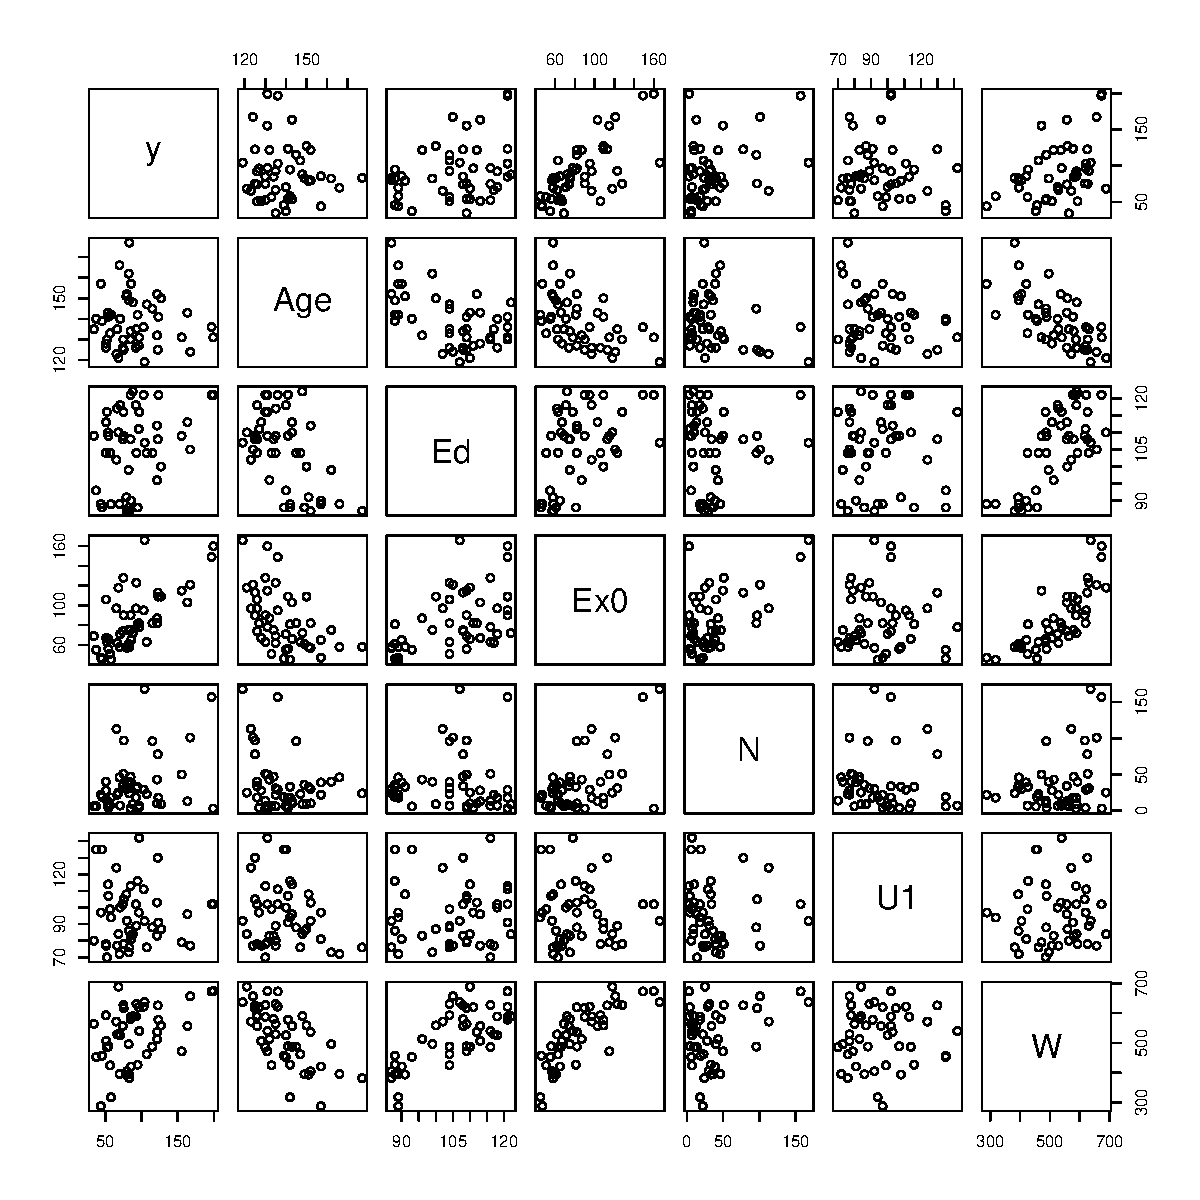
\includegraphics[width=.98\textwidth]{USCrime-scm.pdf}
\end{figure}

\begin{verbatim}
> 
> ##### BLOCK 2 #####
> 
> # Let's fit a model with the intercept only.
> z <- lm.fit(x = X[, 'Const', drop = FALSE], y = y)
>     # Selecting a single row or col will return a simple vector
>     # by default; use 'drop = FALSE' will keep it a matrix.
>     # 'drop' means dropping the dimension info.
> print(coef(z))
   Const 
90.50851 
> 
> # We know this estimate should equal the mean.
> # Does it?
> print(mean(y))
[1] 90.50851
> 
> # Calc SSR and SSE.
> print(ssr.Const <- sum(fitted(z) ^2))    # SSR
[1] 385014.2
> print(sse.Const <- sum(residuals(z) ^2)) # SSE.
[1] 68809.28
>     # This should equal syy. Does it?
> print(syy)
[1] 68809.28
> print(ssr.Const + sse.Const)
[1] 453823.4
>     # This should equal sstotal. Does it?
> print(sstotal)
[1] 453823.4
> 
> # Let's test the significance of this 'pure-intercept' model.
> print((ssr.Const / 1) / (sse.Const / (n - 1)))
[1] 257.3875
> print(qf(1 - alpha, 1, n - 1))
[1] 4.051749
>     # Is the test statistic greater than the critical value?
>     # Is it surprising to you that the intercept is significant?
> 
\end{verbatim}

\begin{verbatim}
> 
> 
> ##### BLOCK 3 #####
> 
> # Let's add predictor 'Age'.
> z <- lm.fit(x = X[, c('Const', 'Age')], y = y)
> print(coef(z))
      Const         Age 
128.6645573  -0.2753469 
> 
> # Calc SSR and SSE.
> print(ssr.ConstAge <- sum(fitted(z) ^2))    # SSR
[1] 385565
> print(sse.ConstAge <- sum(residuals(z) ^2)) # SSE.
[1] 68258.44
> print(ssr.ConstAge + sse.ConstAge)
[1] 453823.4
>     # This should equal sstotal. Does it?
> print(sstotal)
[1] 453823.4
> 
> # Let's test the significance of the coef for 'Age'.
> print(((ssr.ConstAge - ssr.Const)/ 1) / (sse.ConstAge / (n - 2)))
[1] 0.3631461
> print(qf(1 - alpha, 1, n - 2))
[1] 4.056612
>     # Is the test statistic greater than the critical value?
> 
> # Turns out to be insignificant.
> # Compare the sse's:
> print(sse.Const)
[1] 68809.28
> print(sse.ConstAge)
[1] 68258.44
>     # The decrease is indeed small.
> 
> # ssr.ConstAge - ssr.Const should be equal to
> # sse.Const - sse.ConstAge.
> # Is it?
> print(ssr.ConstAge - ssr.Const)
[1] 550.8396
> print(sse.Const - sse.ConstAge)
[1] 550.8396
>     # Both are SSR(Age | Const)
> 
> # Out of curiosity,
> # is the extra SS of 'Age' the same as the SSR of 'Age' alone?
> z <- lm.fit(x = X[, 'Age', drop = FALSE], y = y)
> print(ssr.Age <- sum(fitted(z) ^ 2))
[1] 379351.5
> 
> # Compare the above with SSR(Age | Const).
> # The SSR of 'Age' alone is much larger than its extra contribution
> # on top of 'Const'.
> 
> # Now, adding 'Age' on top of 'Const' is not significant.
> # Does 'Age' alone makes a significant model?
> sse.Age <- sum(residuals(z) ^ 2)
> print( (ssr.Age / 1) / (sse.Age / (n - 1)) )
[1] 234.3188
> print(qf(1 - alpha, 1, n - 1))
[1] 4.051749
>     # Is the test statistic greater than the critical value?
> 
\end{verbatim}

\begin{verbatim}
> 
> ##### BLOCK 4 #####
> 
> # Does 'Const' and 'Age' as a group make a significant model?
> # The answer must be 'yes', given the preceding results.
> # But let's do a test anyway.
> # The things we need are already computed.
> print( (ssr.ConstAge / 2) / (sse.ConstAge / (n - 2)) )
[1] 127.0936
> print(qf(1 - alpha, 2, n - 2))
[1] 3.204317
>
\end{verbatim}

\begin{verbatim}
> ##### BLOCK 5 #####
> 
> # Keeping 'Const' and 'Age' in the model,
> # let's add 'Ed' and 'Ex0' at once.
> z <- lm.fit(x = X[, c('Const', 'Age', 'Ed', 'Ex0')], y = y)
> print(coef(z))
       Const          Age           Ed          Ex0 
-221.0878571    1.2300299    0.4737244    1.0717904 
> 
> ssr.CAEE <- sum(fitted(z) ^ 2)
> sse.CAEE <- sum(residuals(z) ^ 2)
> print(ssr.CAEE + sse.CAEE)  # This should be equal to 'sstotal'.
[1] 453823.4
> print(sstotal)
[1] 453823.4
> 
> # Let's test the group.
> print( ((ssr.CAEE - ssr.ConstAge) / 2) / (sse.CAEE / (n - 4)) )
[1] 28.65531
> print(qf(1 - alpha, 2, n - 4))
[1] 3.214480
> 
> 
\end{verbatim}

\end{document}

